\documentclass[12pt]{article}
% \textwidth 15.5cm \oddsidemargin 0cm \topmargin -2cm \textheight
% 24cm \footskip 1cm
\usepackage[british]{babel}
\usepackage{epsfig}
\usepackage{amsmath,graphicx,psfrag,pstricks,float,amssymb,fancyhdr,pdfpages, hyperref, enumitem, listings, subcaption, minted, diagbox, appendix, lastpage}
\usepackage[sorting=none]{biblatex}
\usepackage[margin=25mm]{geometry}

% \pagestyle{fancy}
% \pagenumbering{arabic}
% \fancyhead[L]{}
% \cfoot{\thepage}
\pagestyle{fancy}
\fancyhf{}
\fancyfoot[C]{Page \thepage\ of \pageref{LastPage}}
% \setlength{\headheight}{15pt}
\renewcommand{\headrulewidth}{0pt}
\linespread{1.3}  % "One-and-a-half" spacing

\def\n{\noindent}
\def\u{\underline}
\def\hs{\hspace}
\newcommand{\thrfor}{.^{\displaystyle .} .}
%\newcommand{\bvec}[1]{{\bf #1}}

\addbibresource{bibliography.bib}

\begin{document}

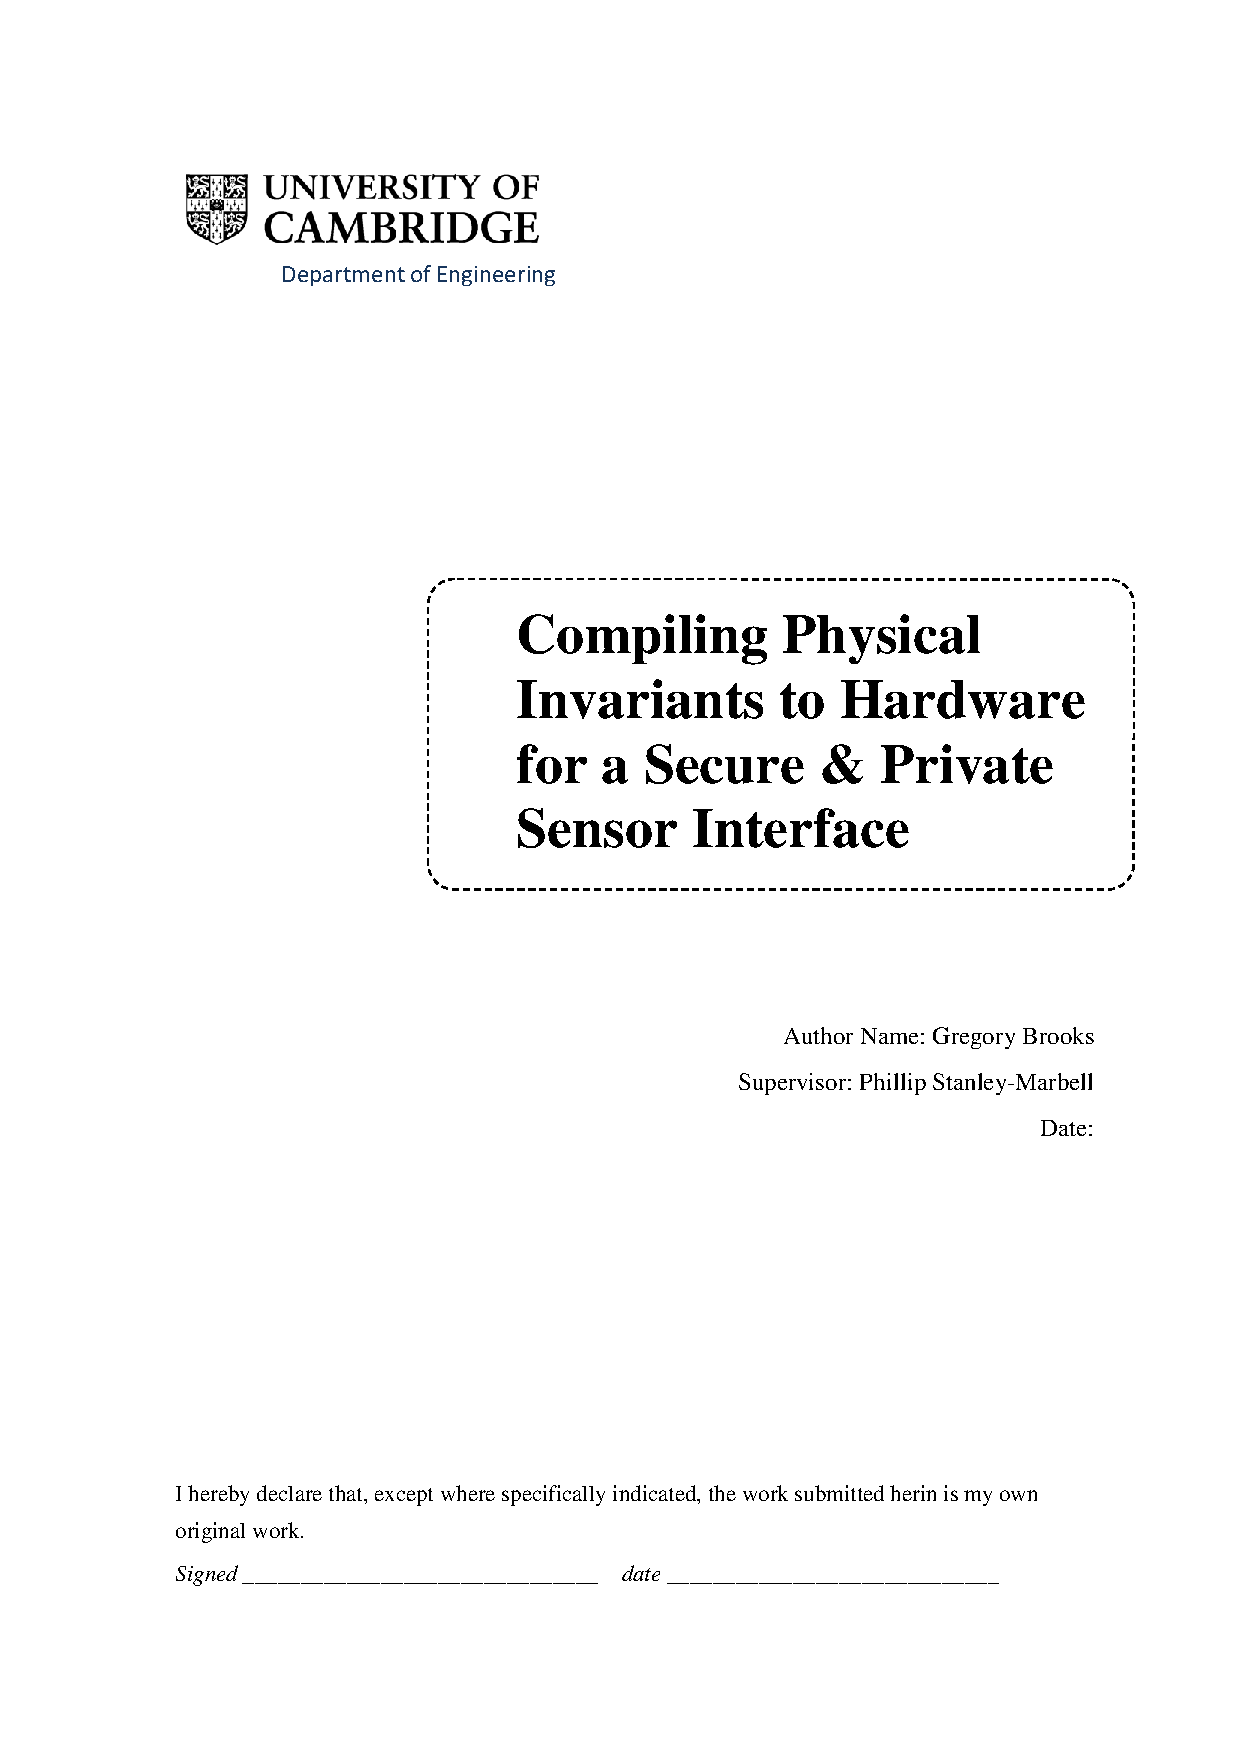
\includepdf[pages={1}]{coversheet.pdf}
\clearpage \mbox{}
\pagenumbering{gobble}
\clearpage
\pagenumbering{arabic}

\noindent

%
% TITLE & CONTENTS PAGE
%

\title
{
  IIB Project Report:\\
  Compiling Physical Invariants to Hardware for a Secure \& Private Sensor Interface\\
}
\author{Gregory Brooks, gb510, Christ's College}
\date{}
\maketitle

\tableofcontents

\pagenumbering{gobble}
\clearpage
\pagenumbering{arabic}

%
% TECHNICAL ABSTRACT
%

\section{Technical Abstract}

\begin{center}
{
  \bf Compiling Physical Invariants to Hardware for a Secure \& Private Sensor Interface\\
}
Gregory Brooks, gb510, Christ's College
\end{center}
\rule{15.7cm}{0.5mm}
\vspace{1cm}


\textit{$\langle$ TODO: write this last$\rangle$}

\newpage



% \clearpage
%
% INTRODUCTION
%

\section{Introduction}

\newpage



%
% THEORY AND DESIGN OF EXPERIMENT
%

\section{Theory And Design of Experiment}

\newpage



%
% APPARATUS AND EXPERIMENTAL TECHNIQUES
%

\section{Apparatus and Experimental Techniques}

\newpage



%
% RESULTS AND DISCUSSION
%

\section{Results and Discussion}

\newpage



%
% CONCLUSIONS
%

\section{Conclusions}

\newpage



\noindent

% Hack to remove REFERENCES REFERENCES header
\markboth{}{}
\printbibliography
\markboth{}{}

\begin{appendix}
\end{appendix}

\end{document}
